\section{Architettura generale di un dispositivo di I/O}
In generale un dispositivo di I/O può essere visto come l'insieme di tre parti fondamentali:

\begin{itemize}

    \item \textbf{Registri Dato, Stato e Controllo}: Tali registri sono quelli che interagiscono in maniera diretta con la CPU, e vengono utilizzati da quest'ultima per controllare e gestire le informazioni del dispositivo. Tali registri sono presenti internamente all'architattura del Calcolatore (ad esempio sulla scheda madre);

    \item \textbf{Sistema di adattamento}: Il sistema di adattamento adatta i segnali provenienti dal mondo esterno per essere letti o scritti nei registri di Dato, Stato e Controllo, e quindi permette di adattare l'attacco esterno (tipo l'USB che utilizza comunicazioni sequenziali), con la comunicazione parallela che il processore ha con i registri;

    \item \textbf{Mondo esterno}: Per mondo esterno si intende tutta la parte che interagisce con il dispositivo in maniera fisica, ed il dispositivo fisico stesso. (immagina una tastiera con il suo connettore USB).

\end{itemize}

Un esempio di dispositivo esterno è la memoria HDD.
La memoria HDD ha difatti i tre registri di Dato, Stato e Controllo: nel processo di scrittura in memoria, la CPU modifica i suddetti registri. Mentre la CPU modifica tali dati, il sistema di adattamento converte i dati presenti in quei tre registri in movimenti della testina + scrittura, rispettando sempre i controlli dati dalla CPU. La scrittura/lettura dei dati tramite la testina e la testina stessa rappresentano, invece, il mondo esterno.
Un altro esempio di periferica è la classica porta \textbf{UART}, che trasmette i sui dati in serie, ma il suo controllo avviene in parallelo. Pertanto al suo interno avrà sia un timer per scandire il clock in base alla tipologia di comunicazione, e poi avrà un buffer parallelo-serie, che converte l'informazione da trasmettere in tanti bit seriali. Oltre alla parte parallelo-serie sarà anche dotato di una parte serie-parallelo, nel caso della ricezione.


\subsection{Modalità di comunicazione}
Le tipologie di collegamento che si possono avere tra un processore e le sue periferiche sono le seguenti:
\begin{itemize}
    \item \textbf{Collegamento passivo}: la periferica e la CPU non condividono alcun tipo di comunicazione. Quindi la CPU presuppone che la periferica sia sempre pronta ed è quindi solo lei a decidere quando e come utilizzare i dati, anche se questi magari non sono pronti o ben processati;
    \item \textbf{Collegamento Sincrono}: La periferica e la CPU comunicano tramite un clock di riferimento per entrambe;
    \item \textbf{Collegamento con Handshacking}: L'handshacking è una modalità di comunicazione asincrona, poichè si sfruttano dei segnali di comunicazione tra la CPU e la periferica che permettono di sincronizzare le operazioni. Una classica implementazione è quella del segnale di \textit{req} che viene alzato dal processore per far capire che vuole leggere e dall'\textit{ACK} alzato dalla periferica che fa comprendere che il dato è pronto o che è stata presa in carico una determinata operazione richiesta. La differenza con la comunicazione sincrona è l'assenza di base dei tempi comune (clock);
    \item \textbf{Collegamento semisincrono}: La trasmissione dei dati è controllata da una base dei tempi comune, ma vengono usati anche segnali di sincronizzazione aggiuntivi (segnali di start e allineamento periodico) per mantenere la sincronizzazione tra trasmettitore e ricevitore;
\end{itemize}

\subsection{Interfacciamento CPU e periferica}
Per utilizzare le periferiche la CPU deve poter accedere ai registri di Dato, Stato e Controllo di tali periferiche. Le tipologie di interfacciamento che ci possono essere tra CPU e Periferica sono:
\begin{itemize}
    \item \textbf{Memory Mapped I/O}: La CPU fa riferimento ai registri di Dato, Stato e Controllo di una periferica come se fossero dei registri in memoria;
    \item \textbf{I/O Mapped}: La CPU dispone di specifici codice operativi per interagire con le periferiche di I/O;
\end{itemize}

Nel nostro caso, il Motorola 68k è una tipologia di architettura \textbf{memory mapped}, e quindi la trattazione dei registri avviene mediante i codici operativi di accesso ai registri della memoria. 

\subsubsection{Memory Mapped I/O}
Nel caso di interfacciamento con una struttura Memory Mapped, l'accesso ai registri di una determinata periferica avvengono tramite bus di collegamento. Ciò rappresenta un limite nell'uso degli indirizzi, poichè quando faccio riferimento ad un registro di una periferica, tale indirizzo non deve appartenere al set di indirizzi della memoria centrale.

\subsubsection{I/O Mapped}
Nel caso di interfacciamento con una struttura I/O Mapped, l'accesso ai registri di una determinata periferica avviene mediante degli specifici comandi. Questo perchè le periferiche sono collegate a bus dedicati o hanno una gestione dedicata, che quindi differisce dalle comunicazioni che avvengono in generale all'interno dell'architettura al costo di avere meno modi di indirizzamento, dato che non si userà più la MOVE che è un codice operativo \textit{ortogonale}.

\subsubsection{Logiche di selezione}
Nel processo di selezione di una periferica collegata alla cpu tramite un bus, vengono utilizzati degli indirizzi per realizzare una tra queste logiche:
\begin{itemize}
    \item \textbf{Logica tristate}: è una logica che disconnette la periferica dal bus dati quando non riconosce il proprio indirizzo. In questo stato, la periferica non interferisce con le comunicazioni e ignora qualsiasi variazione presente sul bus. La logica tristate si basa sull'indirizzo interno assegnato alla periferica stessa. Si definisce \textit{tristate} perchè un'uscita può trovarsi in tre stati logici:
    \begin{itemize}
        \item \textbf{0}: livello basso;
        \item \textbf{1}: livello alto;
        \item \textbf{Alta impedenza}: praticamente disconnesso; 
    \end{itemize}
    \item \textbf{Logica Plug-and-play}: in questo caso, l'indirizzo della periferica non è fisso, ma viene selezionato dinamicamente tra un insieme di indirizzi disponibili. Questo consente di configurare automaticamente in fase di inizializzazione le periferiche senza dover intervenire manualmente per impostare l'indirizzo.
\end{itemize}

\subsection{BUS}
I bus sono responsabili del collegamento tra le varie componenti di un calcolatore (CPU, memoria e periferiche di I/O).
In generale, le tipologie di bus variano in base all'applicazione e alla tecnologia utilizzata. I bus si contraddistinguono principalmente per la divisione che attuano sui loro collegamenti, ma in generale, le informazioni che vengono trasportate sono le stesse.
Queste sono dipartite tra i vari collegamenti presenti in un BUS. I collegamenti generici che si possono identificare in un bus sono:
\begin{itemize}
    \item \textbf{Alimentazione}: Collegamenti che principalmente comprendono la VCC (o più VCC), che sarebbero le tensioni di alimentazione delle componenti, ed il cavo di terra (o GND);
    \item \textbf{Dati}: Collegamenti che trasportano i dati che vengono scambiati tra i vari dispositivi;
    \item \textbf{Indirizzo}: Collegamenti che trasportano gli indirizzi che permettono la selezione dei dispositivi interessati o dei registri a cui si vuole accedere in lettura o scrittura;
    \item \textbf{Controllo}: Collegamenti che trasportano le informazioni inerenti alla tipologia di operazione che si vuole effettuare;
    \item \textbf{Stato}: Collegamenti che permettono il controllo di flusso e la segnalazione di eventuali conflitti o errori;
\end{itemize}

Data una tipologia di bus, può succedere che la periferica considerata non è compatibile con quella determinata tipologia di bus. Pertanto, si può considerare l'uso di un \textbf{adapter}, che mi permette di adattare il bus classico con la tipologia di attacco specifica per la mia periferica. Oltretutto in alcuni casi, quando il dispositivo non permette la configurazione degli indirizzi, per evitare conflitti, l'adapter gestisce anche la gestione di tale indirizzo rispetto al sistema.

\subsection{Driver}
I driver sono dei software di basso livello che consentono di tradurre le richieste delle applicazioni per le periferiche in comandi specifici comprensibili dall'hardware. Ogni tipo di periferica necessita del proprio driver, e spesso è fornito dal costruttore dell'hardware stesso. 
Nella programmazione di un driver si possono seguire vari approcci in base al modo in cui vengono gestiti i tempi e le modalità di comunicazione con la CPU. L'approccio più semplice e primitivo è il \textbf{Polling}. Questo approccio consiste nel dare un primo segnale di controllo alla periferica e si \textit{aspetta} uno specifico valore di stato per poter accedere al dato. Questo sistema è tuttavia inefficiente, poichè mentre la CPU aspetta la riposta della periferica si sprecano dei periodi di clock nei quali la CPU non esegue operazioni utili. Lo stato in cui la CPU permane senza eseguire delle operazioni utili è detto \textbf{Busy-waiting}. Un possibile codice di implementazione di questo tipo di approccio è [\ref{m68:polling}]:

\begin{lstlisting}[caption={Codice polling}, label=m68:polling]
        ORG     $8000  * Inizializzazione registri
        MOVE.B  #$00,C
        MOVE.B  #$00,S
        MOVEA.L #VAR1,A0
        MOVE.W  #0,D0
FOR     CMP.W   #N,D0   * N byte da ricevere
BGE   FUORI
* Codice Driver:
        MOVE.B  #$01,C  * Set del controllo
L1      MOVE.B  S,D1    * Inizio ciclo polling
        AND.B   #$80,D1  
* Se il bit si e' alzato ho finito. 
* Altrimenti continuo ad aspettare
        BEQ     L1
        MOVE.B  D,(A0)+ *Inserisco il dato in memoria
        MOVE.B  #$00,C  *Reset segnale di Controllo
        MOVE.B  #$00,S  *Reset Segnale di stato 
        ADD.B   #1,D0             
        BRA     FOR
FUORI
        ORG     $8100
D       DS.B    1   *Registro dato
S       DS.B    1   *Registro Stato
C       DS.B    1   *Registro Controllo
N       EQU     5   *Dimensione array da trasferire
VAR1    DS.B    5   *Array effettivo di raccolta dati
\end{lstlisting}
\newpage
Il codice [\ref{m68:polling}] presenta però le seguenti criticità:
\begin{itemize}
    \item \textbf{Mancata Generalizzazione}: Si vanno a considerare in maniera diretta i registri in memoria D,S,C che per l'implmentazione di un driver riutilizzabile non è una scelta corretta. Diverse istanze della stessa periferica (collegate quindi ad indirizzi diversi) avrebbero bisogno di un driver diverso;
    \item \textbf{Polling}: L'attesa che viene svolta all'interno di tale codice non permette al processore di eseguire altre operazioni prima di aver ricevuto tutti i caratteri;
    \item \textbf{Gestione dei malfunzionamenti}: Se la periferica ha un qualunque tipo di malfunzionamento e quindi non aggiorna mai il registro di stato, tale ciclo eseguirà all'infinito senza mai fermarsi.
\end{itemize}

Le due criticità possono essere risolte in diversi modi. La soluzione alla prima problematica è molto semplice: al posto di considerare i registri di Dato, Stato e Controllo in maniera diretta, possono essere considerati come registri indirizzo (Ai), a cui vado ad associare gli indirizzi di tali registri. Tali inidirizzi poi vengono settati secondo un determinato criterio prima della chiamata al driver.
Per ovviare al secondo problema c'è il bisogno di considerare le \textbf{interruzioni}. Per l'ultimo problema la soluzione è l'introduzione di \textbf{timer}, che permettono di capire quando un sistema sta impiegando un tempo più grande del dovuto per eseguire un' operazione, e ciò permette di poter gestire situazioni indesiderate di attesa indefinita.

\subsection{PIA} \label{par:PIA}

La \textbf{PIA (Periferal Interface adapter)} è un dispositivo di comunicazione parallela ad 8 bit. Tale architettura è un dispositivo hardware che si posiziona tra la periferica e il processore stesso. Essa è costituita architetturalmente da due tipologie diverse di porto, il porto A ed il porto B.[\ref{img:PIA}]
Tali porti hanno dei registri che sono direzionali, quindi possono assumere una sola funzione (tra entrata ed uscita), in base alla loro configurazione.
% Prima di parlare di più porti ci concentriamo sulle comunicazioni a singolo porto; in generale le comunicazioni che avvengono tra due interfacce della PIA sono configurabili tramite i bit di configurazione del chipset. Nel nostro caso, la comunicazione che maggiormente utilizzeremo è quella dotata di handshacking, per cui si avrà una configuraizone ed un collegamento simile all'immagine [\ref{img:PIA-CON}].
Facendo riferimento alla figura \ref{img:PIA}, osserviamo che il dispositivo si interfaccia al MC68K con un bus dati a 8 bit bidirezionale, tre linee di \textit{chip select} CS, due linee di \textit{register select} RS, una linea di controllo per indicare un'operazione di lettura e scrittura RW, due linee di \textit{interrupt request} IRQ, una linea di \textit{enable} e una linea di \textit{reset}. 
Il bus dati a 8 bit bidirezionale permette il trasferimento di dati tra il processore e la PIA, e i collegamenti seguono la logica \textit{three state}, ovvero permangono in uno stato di alta impedenza (off) tranne quando il processore performa una lettura su questi 8 bit. 
La linea enable costituisce l'unico segnale di timing fornito al dispositivo. La linea RW trasmette un segnale generato dal processore per controllare la direzione del trasferimento dati sul bus. Per selezionare il dispositivo, le linee CS0 e CS1 devono essere alte mentre la linea $\overline{CS2}$ deve essere bassa.
Le linee RS sono utilizzate come vedremo tra poco per selezionare registri interni alla PIA in combinazione con i control registers interni alla PIA. Le linee $\overline{IRQA}$ e $\overline{IRQB}$ sono utilizzate in accordo a quanto condfigurato nei registri di controllo per abbassarsi e segnalare alla cpu un'interruzione.
Come si osserva in figura \ref{img:PIA}, lato periferica invece la PIA si interfaccia mediante due bus dati da 8 bit e quattro linee di interrupt/controllo. I due bus dati fanno riferimento al porto A e al porto B della medesima PIA. Per quanto riguarda il porto A, ognuna delle linee può essere programmata per essere input o output. Questo si può fare settando a 1 (output) o 0 (input) il corrispondente bit del \textit{Data direction register} DDRA. Un discorso analogo può essere fatto per il porto B.
Per quanto riguarda le linee CA1 e CB1, sono linee di input utilizzate per settare i bit inerenti ai flag di interrupt dei control registers di A e B. CA2 è una linea che utilizzeremo con direzionalità output, e la funzionalità sarà chiarita dal control register del porto A. Un discorso analogo può essere fatto per CB2.

\subsubsection{Configurazione PIA}
Dopo un segnale di $\overline{RESET}$, tutti i registri della PIA vengono azzerati e segue una fase di configurazione da parte della CPU. In totale, le locazioni accessibili internamente alla PIA sono 6 e illustrate nella tabella \ref{Tab:reg_ind_1}


% Il dispositivo PIA simulato in ASIM è derivato da quello commerciale MC6821. Questo è dotato di sei registri a 8 bit, tra cui: due registri per il trasferimento dei dati da e verso la periferica (\textit{PRA} e \textit{PRB}); due registri di controllo/stato (\textit{CRA} e \textit{CRB}); infine due registri per il controllo della direzione dei dati (\textit{DRA} e \textit{DRB}). Questi registri sono accessibili mediante indirizzamento interno secondo la tabella \ref{Tab:reg_ind_1}:

\begin{table} [ht]
    \centering
    \begin{tabular}{|c|c|c|c|c|}
        \hline
        \multicolumn{5}{|c|}{\textbf{Indirizzamento interno}} \\ \hline
        \textbf{RS1} & \textbf{RS0} & \textbf{CRA2} & \textbf{CRB2} & \textbf{Registro selezionato}\\ \hline
        0       &0      &1      &X      &PRA    \\  \hline
        0       &0      &0      &X      &DRA    \\  \hline
        0       &1      &X      &X      &CRA    \\  \hline
        1       &0      &X      &1      &PRB    \\  \hline
        1       &0      &X      &0      &DRB    \\  \hline
        1       &1      &X      &X      &CRB    \\  \hline
    \end{tabular}
    \caption{Indirizzamento interno}
    \label{Tab:reg_ind_1}
\end{table}

Questi registri sono selezionabili dal processore mediante le linee RS1 ed RS0.
I \textit{Control Register} CRA e CRB permettono al processore di controllare l'operazione delle quattro linee di controllo periferica CA1, CA2, CB1, CB2. Permettono alla CPU inoltre di abilitare le linee di interruzione e controllare lo stato dei flag di interruzione. 
Gli 8 bit del CRA sono commentati in tabella \ref{Tab:control_registers}:

\begin{table}[ht]
    \centering
    \renewcommand{\arraystretch}{1.5} % Aumenta l'altezza delle righe
    \setlength{\tabcolsep}{8pt} % Uniforma la distanza tra colonne
    \begin{tabular}{|c|c|c|c|c|c|c|c|c|}
        \hline
        \multirow{2}{*}{\textbf{CRA}} 
        & \textbf{7}  & \textbf{6}  & \textbf{5}  & \textbf{4}  & \textbf{3}  & \textbf{2}  & \textbf{1}  & \textbf{0}  \\ 
        \cline{2-9} 
        & \textit{IRQA1}  & \textit{IRQA2}  
        & \multicolumn{3}{c|}{\textit{controllo CA2}}  
        & \textit{Accesso DRA}  
        & \multicolumn{2}{c|}{\textit{controllo CA1}}  \\ 
        \hline
        \multirow{2}{*}{\textbf{CRB}}  
        & \textbf{7}  & \textbf{6}  & \textbf{5}  & \textbf{4}  & \textbf{3}  & \textbf{2}  & \textbf{1}  & \textbf{0}  \\ 
        \cline{2-9} 
        & \textit{IRQB1}  & \textit{IRQB2}  
        & \multicolumn{3}{c|}{\textit{controllo CB2}}  
        & \textit{Accesso DRB}  
        & \multicolumn{2}{c|}{\textit{controllo CB1}}  \\ 
        \hline
    \end{tabular}
    \caption{Control Registers}
    \label{Tab:control_registers}
\end{table}

Vediamo nel dettaglio il significato di questi bit nella tabella \ref{Tab:CRA} e nella tabella \ref{Tab:CRB}:
\newpage

\begin{table}[h!]
    \centering
    \begin{tabular}{|c|c|p{9cm}|}
    \hline
    \multicolumn{3}{|c|}{\textbf{CRA}} \\
    \hline
    \textbf{Bit} & \textbf{Valore} & \textbf{Significato} \\
    \hline
    \multirow{2}{*}{0} & 0 & Disabilita la transizione di IRQA allo stato low in seguito ad una transizione attiva di CA1 \\
                    & 1 &  Abilita la transizione di IRQA allo stato low in seguito ad una transizione attiva di CA1 \\
                    \hline
    \multirow{2}{*}{1} & 0 & IRQA1 (bit 7) settato alto su transizioni alto-basso di CA1 \\
                    & 1 & IRQA1 (bit 7) settato alto su transizioni basso-alto di CA1 \\
                    \hline
                    \multirow{2}{*}{2} & 0 & Selezionato DDRA \\
                    & 1 & Selezionato PRA \\
    \hline
    5,4,3 & 100 & Operiamo secondo il procollo handshaking* \\
                    
    \hline
    6 & X & IRQA2 non è affetto dalle transizioni di CA2 quando b5=0\\
    \hline
    7 & 1 & Bit di sola lettura, si alza su transizioni attive di CA1. Viene resettato da una lettura dell'output register A da parte della CPU \\
    \hline
\end{tabular}
    \caption{dettaglio bit CRA}
    \label{Tab:CRA}
\end{table}

\begin{table}[h!]
\centering
\begin{tabular}{|c|c|p{9cm}|}
    \hline
    \multicolumn{3}{|c|}{\textbf{CRB}} \\
    \hline
    \textbf{Bit} & \textbf{Valore} & \textbf{Significato} \\
    \hline
    \multirow{2}{*}{0} & 0 & Disabilita la transizione di IRQB allo stato low in seguito ad una transizione attiva di CB1 \\
                    & 1 &  Abilita la transizione di IRQB allo stato low in seguito ad una transizione attiva di CB1 \\
    \hline
    \multirow{2}{*}{1} & 0 & IRQB1 (bit 7) settato alto su transizioni alto-basso di CB1 \\
    & 1 & IRQB1 (bit 7) settato alto su transizioni basso-alto di CB1 \\
    \hline
    \multirow{2}{*}{2} & 0 & Selezionato DDRB \\
    & 1 & Selezionato PRB \\
    \hline
    5,4,3 & 100 & Operiamo secondo il procollo handshaking* \\
    
    \hline
    6 & X & IRQB2 non è affetto dalle transizioni di CB2 quando b5=0\\
    \hline
    7 & 1 & Bit di sola lettura, si alza su transizioni attive di CB1. Viene resettato da una lettura dell'output register B da parte della CPU \\
    \hline
\end{tabular}
\caption{dettaglio bit CRB}
\label{Tab:CRB}
\end{table}

Un'importante osservazione va fatta sui bit 5,4,3. Durante il corso è stata affrontata il solo caso in cui b5 = 1, ovvero la linea CA2 (CB2) è una linea di \textbf{output}, e il caso in cui b4,b3 = 00, ovvero:
\begin{itemize}
    \item CA2 si abbassa dopo una lettura da parte della CPU dell'output register A, mentre si alza sulla successiva transizione attiva di CA1 come specificato nel bit 1.
    \item CB2 si abbassa dopo una scrittura da parte della CPU sull'output register B, mentre si alza sulla successiva transizione attiva di CB1 come specificato nel bit 1. b7 va innanzitutto resettato con una \textit{lettura fittizia} sull'output register B.
\end{itemize}


\begin{figure}[ht]
    \centering
    % 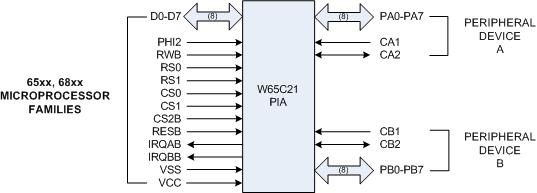
\includegraphics[width=0.45\textwidth]{img/PIA.png}
    % \hfill
    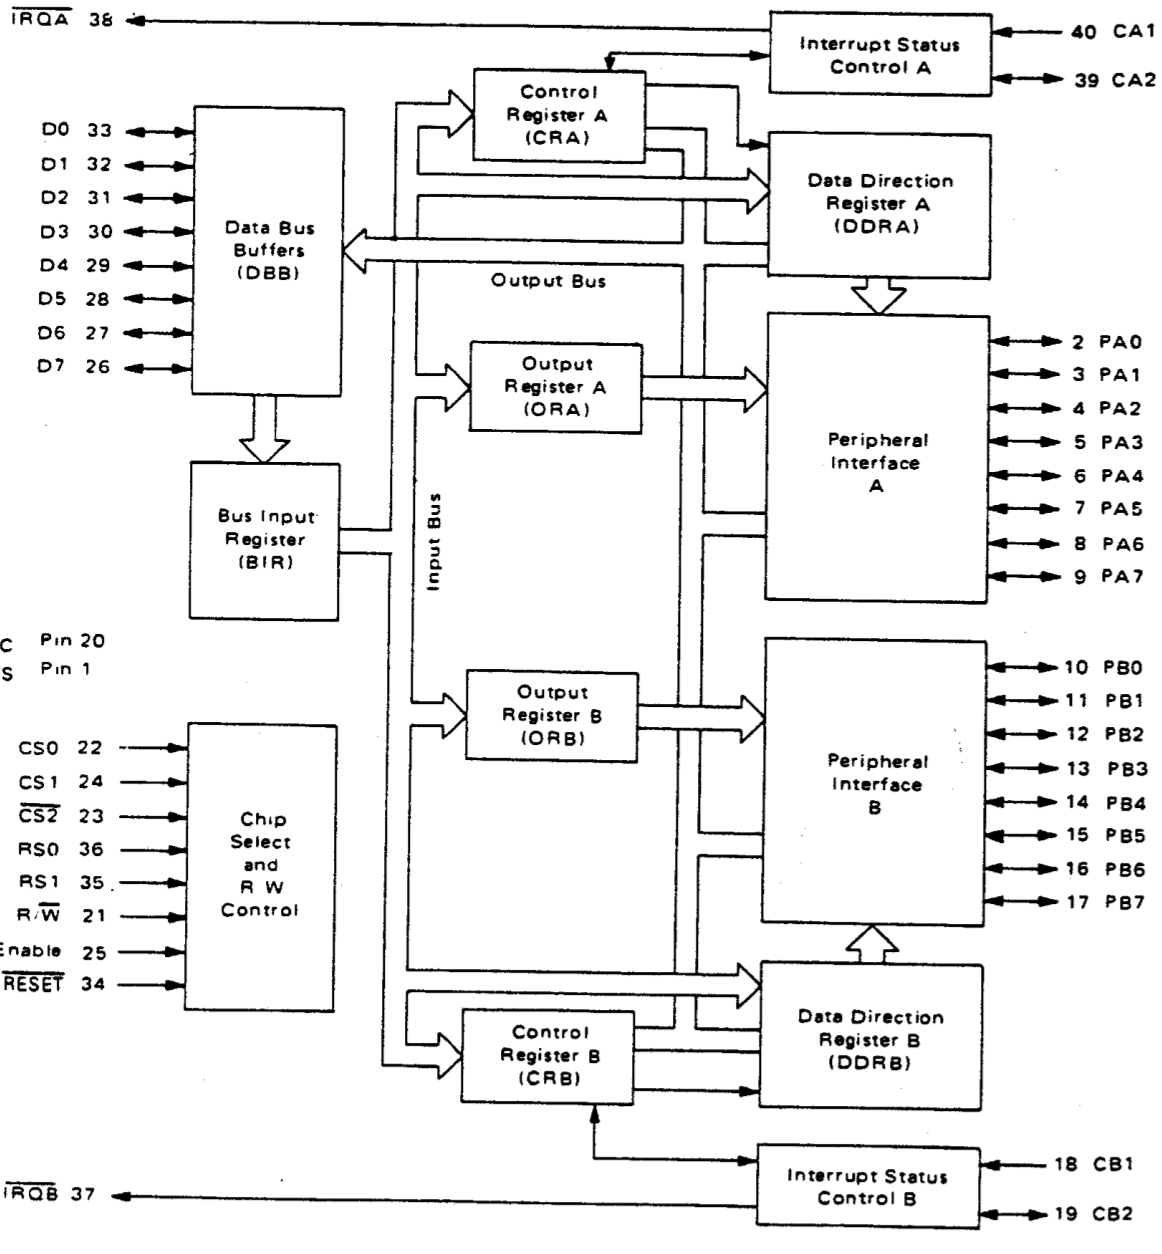
\includegraphics[width=0.9\textwidth]{img/PIA-SCHEME.jpg}
    \caption{Architettura MC68A21CP} \label{img:PIA}
\end{figure}

\subsubsection{Comunicazione tramite PIA}
Per far si che due architetture possano comunicare è quindi importante definire il collegamento e la direzionalità. Una possibile architettura di collegamento è quella visibile nella figura [\ref{img:PIA-CON}].

\begin{figure}
    \centering
    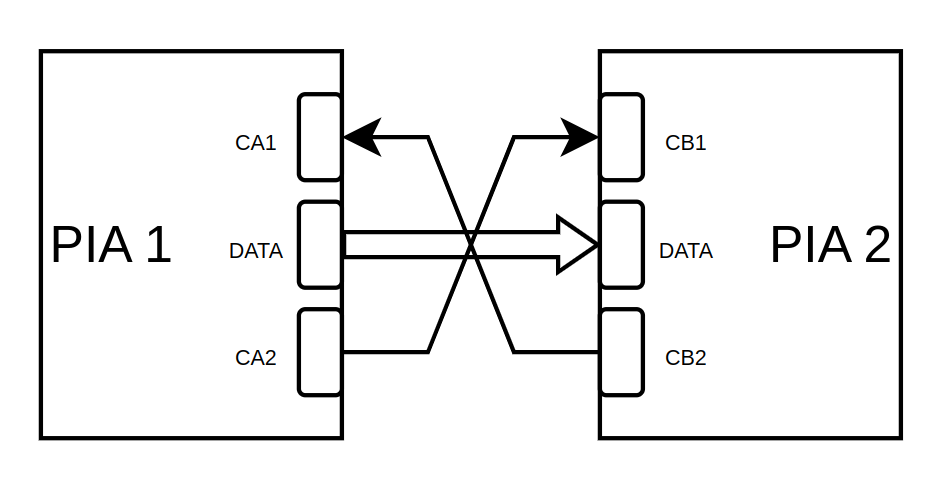
\includegraphics[width=0.65\textwidth]{img/PIA-CON.png}
    \caption{Collegamento tra due dispositivi tramite PIA}\label{img:PIA-CON}
\end{figure}
Durante il corso, gli esercizi sulla PIA sono stati effettuati sfruttando il simulatore ASIM. La PIA simulata in ASIM ha un comportamento quasi del tutto analogo a quello fin qui presentato per il componente reale. Prima di iniziare la configurazione, bisogna caricare su asim un file .cfg che definisce tutti i dispositivi della simulazione e il loro collegamento, compresa una memoria già inizializzata dove sono già mappati i registri appartenenti al modello di programmazione della PIA.
A questo punto, è possibile eseguire il codice del \textit{driver}, che accede al registro di controllo e al registro dati per attuare la logica di comunicazione. 
Riportiamo di seguito i casi in cui si attua una logica di funzionamento tramite polling (e busy waiting della CPU) e tramite interruzione. 

\begin{lstlisting}
    *** LOGICA POLLING INVIO ***
        ORG     $8200
MAIN    JSR     DVBOUT
        MOVEA.L #PIACB,A1 
        MOVEA.L #PIADB,A2
        MOVEA.L #MSG, A0 
        MOVE    DIM, D0
        CLR     D1 
        CLR     D2
INVIO   MOVE    (A2),D1 
        MOVE    (A0)+,(A2)
        ADDQ    #1,D2 
CICLO   MOVE    (A1), D1 
        ANDI    #%10000000,D1 
        BEQ     CICLO
        CMP     D2,D0 
        BNE     INVIO 
LOOP    JMP     LOOP 

DVBOUT  MOVE    #0, PIACB
        MOVE    #$FF, PIADB
        MOVE    #%00100100,PIACB
        RTS

        ORG     $8000
MSG     DC.B    1,2,3,4,5,6
DIM     DC.B    6
PIADB   EQU $2006   * data register B
PIACB   EQU $2007   * data register A
\end{lstlisting}

Questo è il codice relativo al dispositivo addetto alla trasmissione di un messaggio composto da 6 caratteri. 
DVBOUT è il codice del DriVer relativo al porto B della pia con bus dati in uscita (OUT). Questo codice viene subito invocato dal main: innanzitutto, azzera il control register del porto B, e così facendo azzera il bit 2 in modo che il prossimo accesso ad indirizzo pari a PIADB sarà il registro direzione in accordo alla tabella \ref{Tab:reg_ind_1}; dopodichè, il driver scrive la stringa 11111111 all'interno del direction register settando tutte le linee dati in uscita dal porto B; infine, il driver scrive la stringa 00100100 nel registro di controllo: b0,b1 = 00 -> propagazione delle interruzioni disabilitata (infatti stiamo analizzando il caso in cui il trasmettitore agisce in polling e non tramite interruzioni), b2=1 significa che il prossimo accesso ad indirizzo pari a PIADB sarà un accesso al registro dati, b5,b4,b3 = 100 significa che stiamo utilizzando il protocollo handshaking come specificato in tabella \ref{Tab:CRB} (per questo è necessaria la lettura fittizia all'inizio).
Dopodichè il main inizia la procedura di invio, che consiste:
lettura su sul registro dati della PIA, in modo da abbassare il bit 7 di CRB; scrive sul registro dati del porto B, e quest'operazione abbassa CB2 e abbassare di conseguenza CA1, che nella transizione high-low scatena un'interruzione sul porto A dell'altra PIA che dovrà essere gestito, come vedremo in seguito, da un'operazione di lettura; A questo punto, il main inizia un ciclo improduttivo in cui aspetta che il b7 del control register diventi 1 in seguito ad un'operazione di lettura lato ricezione. 
Usciti dal ciclo, si controlla se restano ancora caratteri da trasmettere ed eventualmente si termina entrando nel ciclo caldo. 

\begin{lstlisting}
*** LOGICA POLLING RICEZIONE *** 
        ORG     $8200
MAIN    JSR     DVAIN 
        MOVE.W  SR,D0
        ANDI.W  #$D8FF,D0 
        MOVE.W  D0,SR 
LOOP    JMP     LOOP 

DVAIN   MOVE    #0,PIACA
        MOVE    #0,PIADA 
        MOVE    #%00100101,PIACA
        RTS

        ORG     $8000
MSG     DS      6
DIM     DC      6
COUNT   DC      0
PIADA   EQU     $2004
PIACA   EQU     $2005

        ORG     $8700
INT3    MOVE.L  A1,-(A7)
        MOVE.L  A0,-(A7)
        MOVE.L  D0,-(A7)

        MOVEA.L #PIADA,A1
        MOVEA.L #MSG,A0 
        MOVE    COUNT,D0 
        MOVE    (A1),(A0,D0)
        ADD     #1,D0 
        MOVE    D0,COUNT

        MOVE.L  (A7)+,D0
        MOVE.L  (A7)+,A0 
        MOVE.L  (A7)+,A1
        RTE 
\end{lstlisting}

La ricezione di un carattere sulla PIA è gestita mediante
interruzione di livello 3 (la PIA non supporta le int.vettorizzate in ASIM) che corrisponde al vettore 27 mappato in area ROM alla locazione \$6C: in tale locazione è contenuto l'indirizzo della ISR in RAM (\$8700). All'arrivo dell'interrupt la ISR acquisisce il carattere e lo salva in un'opportuna posizione in memoria.
Il main chiama immediatamente il Driver DVAIN, che accede al direction register del porto A, imposta le linee del data register A come input (stringa di zero), imposta il registro di controllo con la stringa 00100101: b0,b1 = 01 -> propagazione delle interruzioni abilitata, b2=1 significa che il prossimo accesso ad indirizzo pari a PIADA sarà un accesso al registro dati, b5,b4,b3 = 100 significa che stiamo utilizzando il protocollo handshaking come specificato in tabella \ref{Tab:CRA}.
Dopodichè, il main imposta lo status register in modo tale da permettere ogni tipo di interruzione, ed entra in un ciclo caldo dove attende un'interruzione.
La ISR associata a quest'interruzione salva i registri sullo stack, dopodichè acquisisce il carattere con una lettura dal registro dati e questo fa abbassare il b7 di CRA e CA2. CA2 basso comporta una transizione alto-basso di CB1 che corrisponde all'alzarsi del flag CRB7 (data ack).
Dopodichè incrementa i contatori, ripristina i registri e termina. 
Il problema di questo driver è la \textbf{busy wait} in fase di trasmissione, motivo per cui introduciamo la comunicazione parallela tramite PIA sfruttando il meccanismo di interruzione anche in fase di trasmissione.
\\
\begin{lstlisting}
*** LOGICA INTERRUPT INVIO ***
        ORG     $8200
MAIN    JSR     DVBOUT
        MOVE.W  SR,D0 
        ANDI.W  #$D8FF,D0
        MOVE.W  D0, SR 
*** INVIO PRIMO CARATTERE ***
        MOVE.L  PIADB,A0 
        MOVE.L  PIACB,A1 
        MOVE.L  MSG,A2
        MOVE.L  (A0),D0 
        MOVE.L  (A2),(A0)
        MOVE    #1,COUNT
LOOP    JMP     LOOP 

DVBOUT  MOVE    #0, PIACB
        MOVE    #$FF, PIADB
        MOVE    #%00100101,PIACB
        RTS

        ORG     $8000
MSG     DC.B    1,2,3,4,5,6
DIM     DC.B    6
COUNT   DC.B    0
PIADB   EQU $2006   * data register B
PIACB   EQU $2007   * data register A

        ORG     $8800
INT4    MOVE.L  A1,-(A7)
        MOVE.L  A0,-(A7)
        MOVE.L  D0,-(A7)

        MOVEA.L #PIADB,A1 
        MOVEA.L #MSG,A0 
        MOVE    DIM,D0 
        MOVE    COUNT,D1 

        CMP     D1,D0 
        BEQ     FINE 
INVIO   MOVE    (A0,D1),(A1)
        ADDQ    #1,D1 
        MOVE    D1,COUNT 
FINE    MOVE.L  (A7)+,D0 
        MOVE.L  (A7)+,A0
        MOVE.L  (A7)+,A1 
        RTE
\end{lstlisting}

La configurazione effettuata in DVBOUT differisce da quella presentata in precedenza solo dalla stringa scritta nel CRB, in quanto le transizioni attive di CB1 scatenano un'interruzione sul CRB7. Il main attiva dunque le interruzioni agendo sullo status register, e in seguito procede con un primo invio (altrimenti il sistema resterebbe in stallo). Osserviamo che è necessaria sempre la lettura fittizia sul registro dati per abbassare CRB7, in quanto non sappiamo a pripri in che stato si trovi. Il main scrive dunque un carattere sul registro dati, e questo provoca la transizione alto-basso di CB2 che a sua volta provoca la transizione alto-basso di CA1, che quindi setta a 1 il flag CRA7 e scatena un'interruzione che gestisce il dispositivo ricevitore: questo farà una lettura sul registro dati del porto A, e questo comporterà l'abbassamento di CRA7 e di CA2, che comporterà l'abbassamento di CB1, che scatenerà un'interruzione su CRB7. Questa interruzione sarà gestita dalla ISR4. 

\begin{lstlisting}
*** LOGICA INTERRUPT RICEZIONE ***
        ORG     $8200
MAIN    JSR     DVAIN 
        MOVE.W  SR,D0 
        ANDI.W  #$D8FF,D0 
        MOVE.W  D0,SR 
LOOP    JMP     LOOP 

DVAIN   MOVE    #0,PIACA
        MOVE    #$00,PIADA
        MOVE    #%00100101,PIACB
        RTS

        ORG     $8000
MSG     DS.B    6
DIM     DC.B    6
COUNT   DC.B    0
PIADB   EQU $2006   * data register B
PIACB   EQU $2007   * data register A

        ORG     $8700
INT3    MOVE.W  A1,-(A7)
        MOVE.W  A0,-(A7)
        MOVE.W  D0,-(A7)
        MOVE.W  D1,-(A7)
        MOVE    DIM,D0 
        MOVE    COUNT,D1 
        MOVEA.L #PIADA,A1 
        MOVEA.L #MSG,A0 
        MOVE    (A1),(A0,D0)
        ADDQ    #1,D1 
        MOVE    D1,COUNT

        MOVE.L  (A7)+,D1 
        MOVE.L  (A7)+,D0 
        MOVE.L  (A7)+,A0
        MOVE.L  (A7)+,A1 
        RTE
\end{lstlisting}

In questo esempio non cambia nulla dal caso precedente. 
Per ulteriori esercizi ed esempi, consultare il capitolo \ref{par:Esercitazioni}.
\newpage
% \subsubsection{Comunicazione parallela tramite PIA}
% Entrando nei dettagli del processo di comunicazione, bisognerà fare particolare attenzione ai seguenti registri:
% \begin{itemize}
%     \item \textbf{CA1,CB1}: Sono registri che possono assumere solo direzione di ingresso e solitamente vengono usati come "lettori" di segnali SYN o segnali ACK da parte dell'altro dispositivo;
%     \item \textbf{CA2,CB2}: Sono i registri che possono essere configurati(sia di ingresso che di uscita), ed in generale, in base al protocollo che si vuole interpretare, vengono settati in una determinata modalità di funzionamento (dipendente dalla tipologia di protocollo che si vuole implementare);
%     \item \textbf{Dato}: Il bus dati trasmette parallelamente i dati tra le due periferiche in base al protocollo di comunicazione utilizzato. I bus dati sono unidirezionali, ma la direzione è programmabile. 
% \end{itemize}


% Una volta definita la tipologia di architettura si va a decidere come queste periferiche dovranno interagire tra loro (definizione del protocollo), per cui si va ad impostare uno specifico registro di configurazione che permetterà di impostare le seguenti opzioni:

% \begin{itemize}
%     \item \textbf{Interrupt o polling}: A che livello di priorità si andrà ad impostare l'interruzione della PIA;
%     \item \textbf{Modalità di funzionamento}: se attuo l'handshacking o altre tipologie di protocolli;
%     \item \textbf{Lettura o scrittura}: 

 
% \end{itemize}
% Una volta definita la struttura del registro di configurazione questo viene settato per impostare la PIA. 
% Una volta impostato il modo di funzionamento si va a gestire il tutto. Qundi, se si è scelto un funzionamento tramite interrupt si avrà un certo tipo di comportamento, altrimenti se ne avrà un altro.

% Il funzionamento generale della fase di \textbf{handshaking} tra due dispositivi PIA è gestita, per i nostri esempi, in un particolare modo.
% Per fare chiarezza andremo a dividere la fase di ricezione dalla fase di trasmissione.
% In fase di \textbf{trasmissione} le operazioni che si vanno ad effettuare sonno le seguenti:
% \begin{itemize}
%     \item \textbf{Inserimento del dato}: La periferica posiziona il dato sul bus dati collegato in maniera diretta con la PIA. Una volta effettuato l'inserimento, la periferica tramite la linea CA1 invia un segnale di \textit{dato pronto} alla PIA, quindi sulla transizione di CA1, in accordo alla configurazione, si propaga un'interruzione al processore. Internamente, la periferica alzerà CA2 (in accordo al protocollo handshaking 100);
%     \item \textbf{Attesa dell'ack}: Il sistema aspetta che l'ack si abbassi per capire che il dato è stato inviato correttamente. Una volta ottenuto l'ACK, la PIA abbassa (dopo una lettura fittizia) CA2, che viene interpretato dalla periferica come \textit{registro dati libero};
%     \item \textbf{Lettura fittizia}: Dato che voglio inviare un nuovo dato, ho bisogno di abbassare il bit CRA7, ma non posso farlo in maniera diretta (configurando un apposito registro di controllo), poichè il bit CRA7 è buona norma che sia in sola lettura. Di conseguenza per abbassare tale valore vado ad effettuare una lettura a vuoto (o lettura fittizzia), che mi permette di abbassare il bit CRA7 e la linea CA2 in modo da poter proseguire nelle operazioni;
% \end{itemize}

% Nella fase di ricezione, invece, si ha:
% \begin{itemize}
%     \item \textbf{Attesa del dato}: Si attende che venga inviato un dato sul porto della PIA, tale attesa può essere effettuata o tramite Polling, andando a controllare in continuazione il valore del bit CRB7, o attivando un'interrupt diretta all'arrivo dell'evento sul bit CB1.
    
%     \item \textbf{Ricezione del dato}: Una volta compreso che vi è un dato pronto, si effettua una lettura del dato, ed in automatico, la PIA abbasserà il bit CRB7 ed invierà un segnale di ACK, abbassando il valore in CB2

%     \item \textbf{Fine}: Nel caso di polling, il sistema continuerà ad aspettare nuovi dati andando a controllare il bit CRB7. Mentre nel caso elle interrupt continuerà il suo normale flusso di esecuzione
% \end{itemize}

% Andando ad analizzare il codice delle varie operazioni è importante capire la metodologia di funzionamento del sistema, sia per costruire l'architettura in maniera adeguata che per scrivere i driver in maniera corretta.

% \subsubsection{Configurazione della PIA}
% La PIA prima di essere utilizzata, richiede una propria configurazione, in parte dipendente dall'architettura e da una parte inerente al driver che si deve implementare.
% Per la parte hardware dobbiamo scrivere (almeno per le nostre simulazioni in ASIM), il \textbf{file di configurazione} che definisce tutti gli specifici collegamenti tra i dispositivi con gli specifici significati. Mentre nel caso di configurazione del driver, una volta definita l'architettura su cui si andrà ad eseguire il codice, si vanno ad impostare i registri di controllo e dato, in modo da poter utilizzare il nostro dispositivo (sia con il polling che con interrupt).

% \paragraph{Definizione dei registri di controllo e dato\\}\label{par:cnt-stt} 
% Il registro di controllo ed il registro di stato vengono inizializzati all'interno della configurazione. Quindi prima di iniziare a scrivere il driver bisogna osservare per bene il file di configurazione. Più precisamente dobbiamo osservare i seguenti due parametri della nostra PIA:
% \begin{itemize}
%     \item \textbf{Address 1}: Indirizzo su cui è mappata la PIA;
%     \item \textbf{Address 2}: Indirizzo del registro di controllo della PIA (dove saranno inserite le configurazioni).
% \end{itemize}

% Una volta osservati tali parametri si inizializzano i registri di dato e controllo nel seguente modo:
% \begin{lstlisting}
% PIADB       EQU     $2006	*indirizzo del registro dato 
% PIACB       EQU     $2007	*indirizzo del registro di controllo
% \end{lstlisting}

% Tali registri saranno utilizzati all'interno delle ISR per poter controllare/comunicare con la PIA, sia per configurarla (in una fase iniziale). Più precisamente andiamo ad effettuare le seguenti due operazioni:
% \begin{itemize}
%     \item \textbf{Configurazione}: dove si imposta il registro di controllo in base a quello che si vuole effettuare, quindi viene impostato nelle fasi iniziali del driver;
%     \item \textbf{Gestione}: Vengono definite le modalità di funzionamento in base alla tipologia di filosofia adottata.
% \end{itemize}

% Un main che è uguale in entrambe le tipologie di comportamento (interruzioni e polling) è il seguente:
% \begin{lstlisting}
% *MAIN
% MAIN	JSR    DVBOUT	*Configurazione della PIA
% \end{lstlisting}

% Per la fase di configurazione, la procedura rimane la stessa a meno della maschera, pertanto viene riportato qui il caso con maschera e saranno riaffrontate le due differenti gestioni all'interno degli appositi paragrafi [\ref{par:PIA-INT}] e [\ref{par:PIA-POL}].
% \begin{lstlisting}
% DVBOUT      MOVE.B      #0,PIACB		*seleziona il registro direzione di PIA porto B 
% MOVE.B      #$FF,PIADB	  		*accede a DRB e pone DRA=1 : le linee di B sono linee di output	
% MOVE.B      #%00100101,PIACB   	*imposta il registro di controllo in base alla sua mappatura
% *								;i bit CRB7 e CRB6 sono a sola lettura	
% RTS
% \end{lstlisting}

% Per capire meglio come impostare il registro di controllo, di seguito è riportata la sua mappatura bit a bit:
% \begin{itemize}
%     \item \textbf{Bit 7}:
%     \item \textbf{Bit 6}:
%     \item \textbf{Bit 5}:
%     \item \textbf{Bit 4}:
%     \item \textbf{Bit 3}:
%     \item \textbf{Bit 2}:
%     \item \textbf{Bit 1}:
%     \item \textbf{Bit 0}: \textcolor{red}{FATTI SPIEGARE IL SIGNIFICATO ED IL NOME DEI VARI BIT}
% \end{itemize}

% Per capire meglio come impostare il registro di controllo, riportiamo di seguito un'analisi più approfondita dei bit dei registri di controllo esposti nella tabella \ref{Tab:control_registers}:
% I bit 0,1 -> di CRA (o CRB) servono a controllare il flag di interruzione IRQA1 (IRQB1) in posizione 7 nella parola di stato-controllo. Lo stato del flag IRQA1 si propaga sulla linea di interruzione IRQA verso il processore generando un'interruzione. In particolare, il bit 0 stabilisce se le interruzioni vengono propagate al processore (valore 1) o se vengono \textit{mascherate} (valore 0), mentre il bit 1 serve a stabilire se l'interruzione viene propagata sul fronte di salita del segnale low->high (valore 1) o sul fronte di discesa high->low (valore 0) di CA1.
% Per i bit 3,4,5 di CRA (o CRB) occorre fare una distinzione: se la linea è stata programmata come linea di ingresso (settando il bit 5 a 0), si comporta come i bit 0,1 con b3 nella funzione di b0 e b4 nella funzione di b1; se la linea è stata programmata come linea di uscita (settando il bit 5 a 1), CA2 (CB2) permette di controllare la periferica tramite la linea CA2. Sono previsti 3 possibili modi di sincronizzazione codificati con i bit b4 e b3, ovvero \textcolor{red}{100 -> Modo Handshake}, \textcolor{green}{101 -> Modo impulsivo} (l'abilitazione di CA2 segue il profilo dell'impulso di un clock) e \textcolor{blue}{11x -> Modo dipendente dal bit 3} (ovvero CA2 alto o basso in base a come viene manualmente settato il bit 3).  



% \subsubsection{Gestione PIA senza Interrupt}\label{par:PIA-INT}
% La gestione senza interrupt sfrutta la tecnica del polling per monitorare volta per volta la struttura dei registri di stato, che quindi mi permette di capire quando agire sul dato o meno. Per effettuare il polling ho bisogno di configurare il registro di controllo in modo da non far attivare le interrupt.
% Seguendo lo schema presente alla fine del paragrafo [\ref{par:cnt-stt}], dovrò impostare come controllo la seguente sequenza: 00100100, dove indichiamo che non vi è bisogno dell'uso delle interrupt. Questa sequenza significa che le interrupt non vengono propagate al processore (b0=0), con le linee AD1 e AD0 si accede al registro dati (b2=1), il protocollo scelto è l'handshaking (b5b4b3 = 100).

% Prendendo in considerazione la prima parte del main, quindi, vado a definire come sub-routine di configurazione la seguente schematica:
% \begin{lstlisting}
% DVBOUT	MOVE.B	#0,PIACB		*seleziona il registro direzione di PIA porto B 
% MOVE.B	#$FF,PIADB	  		*accede a DRB e pone DRA=1 : le linee di B sono linee di output	
% MOVE.B	#%00100100,PIACB   	*imposta il registro di controllo come indicato precedentemente
% 								*i bit CRB7 e CRB6 sono a sola lettura	
% RTS
% \end{lstlisting}

% Una volta impostata la periferica, il polling viene effettuato sul registro di controllo. Di seguito vi è l'esempio di un invio di un dato, dove il controllo sull'ack viene effettuato all'interno di un ciclo, senza considerare l'utilizzo delle interrupt.

% \begin{lstlisting}
% ORG     $8200
% MAIN    JSR    DVBOUT	*inizializza PIA 

%         MOVEA.L	#PIACB,A1	*indirizzo registro di controllo CRB
%         MOVEA.L	#PIADB,A2	*indirizzo registro PRB
%         MOVEA.L	#MSG,A0	*indirizzo area messaggio
%         MOVE.B	DIM,D0	*dim del messaggio

%         CLR	D1	*appoggio
%         CLR	D2	*contatore elementi trasmessi


% INVIO	MOVE.B	(A2),D1            *lettura fittizia da PRB => serve per azzerare CRB7 dopo il primo carattere, altrimenti resta settato con l'ack
%         MOVE.B	(A0)+,(A2)	*carattere corrente da trasferire su bus di PIA porto B: dopo la scrittura di PRB, CB2 si abbassa
% *								*cio' fa abbassare CA1 sulla porta gemella dell'altro sistema generando 
% *								*un'interruzione che coincide con il segnale DATA READY
%         ADD.B		#1,D2		    *incremento contatore elementi trasmessi

% ciclo2	MOVE.B	(A1),D1		*In attesa di DATA ACKNOWLEDGE
%         ANDI.B	#$80,D1				*aspetta che CRB7 divenga 1
%         BEQ	ciclo2

%         CMP	D2,D0	*controllo se ho finito di trasmettere
%         BNE	INVIO

% LOOP  	JMP LOOP	*ciclo caldo dove il processore ha completato la trasmissione	
% \end{lstlisting}


% \subsubsection{Gestione PIA con Interrupt}\label{par:PIA-POL}
% La gestione della pia con il funzionamento dell'interrupt va a sfruttare il meccanismo delle interrupt autovettorizzate, per cui oltre a definire il registro di controllo in un certo modo, dobbiamo caricare all'interno dell'area degli indirizzi autovettorizzati, l'indirizzo della nostra ISR (che si traduce in ASIM nel caricare il file di configurazione della memoria fornito dal professore). Il caricamento dei dati non fa altro che inserire l'indirizzo di memoria della nostra ISR all'interno dell'apposita cella identificata.
% Come prima cosa definiamo il registro di configurazione come: 00100101

% Il codice che va a configurare il registro di controllo è il seguente:
% \begin{lstlisting}
% DVAIN	MOVE.B	#0,PIACA		*mette 0 nel registro controllo cosi' al prossimo accesso a PIADA (indirizzo pari)
% *								*selezionera' il registro direzione del porto A
%         MOVE.B	#$00,PIADA		    ;accede a DRA e pone DRA=0 : le linee di A sono linee di input	
%         MOVE.B	#%00100101,PIACA  	;imposta il registro di controllo come indicato sopra, ponendo IRQA1=1 e IRQA2=1
% *								;i bit CRA7 e CRA6 sono a sola lettura	
% RTS
% \end{lstlisting}

% Oltre alla configurazione, andiamo ad attivare il meccanismo delle interrupt all'interno del processore, ed andiamo ad impostare la modalità utente, in modo da poter visualizzare anche che le ISR vengono eseguite sempre in modalità supervisore. Per capire meglio tale passaggio, di seguito vi è il MAIN:
% \begin{lstlisting}
% MAIN	JSR	DVAIN	*inizializza PIA porto A
            
%         MOVE.W	SR,D0	*legge il registro di stato
%         ANDI.W	#$D8FF,D0 *maschera per reg stato (stato utente, int abilitati)
%         MOVE.W	D0,SR	*pone liv int a 000

% LOOP  	JMP LOOP	*ciclo caldo dove il processore attende interrupt	
% \end{lstlisting}

% Una volta scitto il main ed aver fatto tutte le dovute configurazioni, possiamo osservare la scrittura del driver, che avrà il suo indirizzo di inizio caricato nel sistema delle interrupt autovettorizzate, che in questo caso sarà 8700:
% \begin{lstlisting}
%             ORG $8700		

% INT3        MOVE.L  A1,-(A7)		;salvataggio registri che saranno utilizzati
%             MOVE.L  A0,-(A7)
%             MOVE.L  D0,-(A7)

%             MOVEA.L	#PIADA,A1
%             MOVEA.L	#MSG,A0	*indirizzo area di salvataggio              
%             MOVE.B	COUNT,D0	*contatore corrente degli elementi ricevuti

    
%             MOVE.B 	(A1),(A0,D0)	*acquisisce il carattere e lo trasferisce in memoria
% *						*la lettura da PRA fa abbassare CRA7 e CA2 => nell'altro sistema si abbassa CB1
% *						*cio' corrisponde all'attivazione di CRB7 che funge da DATA ACKNOWLEDGE
    
%             ADD.B	#1,D0
%             MOVE.B	D0,COUNT

%             MOVE.L  (A7)+,D0		*ripristino registri 
%             MOVE.L  (A7)+,A0
%             MOVE.L  (A7)+,A1
            
%             RTE
% \end{lstlisting}

\subsection{Interruzioni}
L'interruzione è un evento che cambia la normale esecuzione di un programma per fargli eseguire prima del codice specifico per la gestione di quella determinata condizione [\ref{img:bootint}]. In generale non è corretto parlare solo di interruzioni, poichè tale termine non comprende o non può comprendere anche il caso in cui le interruzioni vengano scatenate dall'interno per casistiche particolari. Difatti è più corretto fare la seguente suddivisione:
\begin{itemize}
    \item \textbf{Interruzioni}: Segnali che sono a contatto con le periferiche e che permettono alla CPU di interrompersi e di eseguire il codice per la gestione della comunicazione con quella data interfaccia. Le interruzioni sono scatenate, quindi, dal dispositivo che vuole interagire con la CPU
    \item \textbf{Eccezioni}: Funzionano come le interruzioni, con la differenza che vengono scatenate internamente rispetto al processore, quindi non vengono gestite dai dispositivi ma dal programma stesso, tale condizione fa eseguire comunque una ISR, con l'obbiettivo di dover gestire particolari casistiche (es. divisione per 0)
\end{itemize}

\begin{figure}
    \centering
    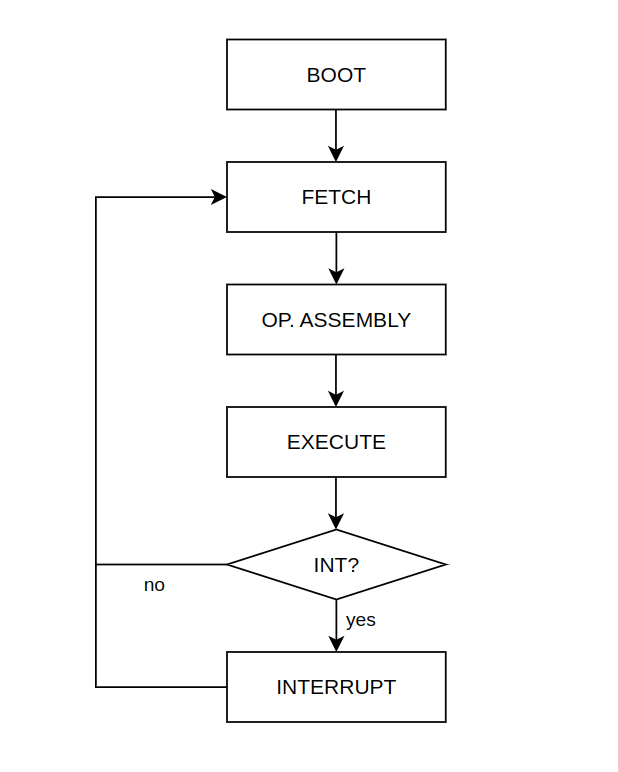
\includegraphics[width=0.5\textwidth]{img/BootInt.png}
    \caption{Ciclo di esecuizone con interrupt}\label{img:bootint}
\end{figure}
Quindi quando le interruzioni sono scatenate vanno ad effettuare una chiamata a subroutine particolare, tale chiamata è detta ISR (Interrupt-Services-Routine). Tale situazione, quindi, ferma il sistema dalla sua normale esecuzione del programma per dare priorità alla gestione dell'interruzione. Questo, quindi, apre molti dubbi su come gestire lo stato in cui si trova la macchina, poichè se quando torno dalla ISR, ho cambiato qualche registro significativo si potrebbe compromettere il normale funzionamento del programma. In generale i due registri che richiedono l'obbligo di essere salvari sono i registri: \textbf{SR(Status register)} e il \textbf{PC(Program Counter)}. In generale, i registri che vado a salvare in questo passaggio sono anche detti: \textbf{Descrittore di processo}, tali registri, quindi, descrivono lo stato di funzionamento del mio processore quando poi è stato prelazionato dalla mia ISR. Ciò mi permette di proseguire ancora con la normale esecuzione del programma prefissato.

\subsubsection{Gestione delle Interruzioni}
Una volta definito cosa sono le interruzioni è di fondamentale importanza capire come il processore le gestisce. Le principali modalità di gestione delle interruzioni sono due e sono:
\begin{itemize}
    \item \textbf{Vettorizzate}: Ogni livello di priorità di interrupt è collegato al processore. I fili di collegamento per le interrupt sono limitati, quindi più dispositivi possono collegarsi sullo stesso cavo di interrupt. Il processore, quindi, per identificare il dispositivo che ha scatenato l'Interrupt va a controllare i bus, su cui il dispositivo ha caricato il suo codice identificativo. Identificare il dispositivo, vuol dire identificare la tipologia di ISR da andare ad utilizzare. Gli indirizzi degli entry-point delle varie periferiche sono memorizzati in memoria a partire dall'indirizzo 0 a seguire per 256 locazioni di 4 byte. Tali locazioni si dividono nel seguente modo:
    \begin{itemize}
        \item \textbf{Funzioni speciali}: Da 0 a 24, gli entry-point identificano delle funzioni speciali o di gestione aritmentica
        \item \textbf{Interruzioni autovettorizzate}: da 25 a 31 sono indicizzate le locazioni per il funzionamento autovettorizzato
        \item \textbf{Trap}: da 32 a 47 sono indicizzate le funzioni per la gestione dei Trap
        \item \textbf{Utilizzabili}: da 48 a 256 sono locazioni disponibili per l'inserimento degli entry-point per la gestione di diverse periferiche
    \end{itemize}
    \item \textbf{Autovattorizzate}: A differenza del caso vettorizzato, evita la lettura del codice identificativo, poichè ogni livello di interrupt è collegato al vettore delle ISR autovettorizzate e permette di selezionare in maniera "ignorante" l'ISR alla locazione della tipologia di priorità inserita
\end{itemize}

\subsubsection{PIC} \label{par:PIC}
In generale, nel caso di sistema \textbf{vettorizzato}, viene in aiuto il componente \textbf{PIC (Programmable Interrupt Controller)} [\ref{img:PIC}].
Il PIC è un dispositivo che permette di arricchire le
modalità di gestione delle interruzioni. Grazie alla programmazione di questo oggetto, possiamo assegnare alle varie periferiche non una sola linea di interruzione con una specifica ISR, ma possiamo esplorare tutto il vettore delle interruzioni, che in teoria è costituito da 256 locazioni. In sostanza, il PIC permette di usare \textbf(interrupt vettorizzate), ovvero il dispositivo fornisce sul data bus un vettore di 8 bit che rappresenta l’indice all’interno della tabella delle interruzioni corrispondente all’indirizzo della corretta ISR. Nel M68k questo protocollo è simulato con il PIC: Il dispositivo non scrive sul data bus il vettore di 8 bit, ma comunica l’interruzione al PIC che si occuperà di capire qual è il vettore corrispondente al dispositivo interrotto. Il PIC estende la gestione delle interruzioni del processore M68K introducendo nuove funzionalità, come la gestione prioritaria, la mascheratura delle interruzioni e le linee di interrupt. Il dispositivo ha in uscita verso il processore una linea di interruzione INT e una linea di INTA (acknowledgement) , mentre ha in ingresso 8 linee di interruzioni differenti, a priorità decrescente (0 massima, 7 minima).

\begin{figure} [ht]
    \centering
    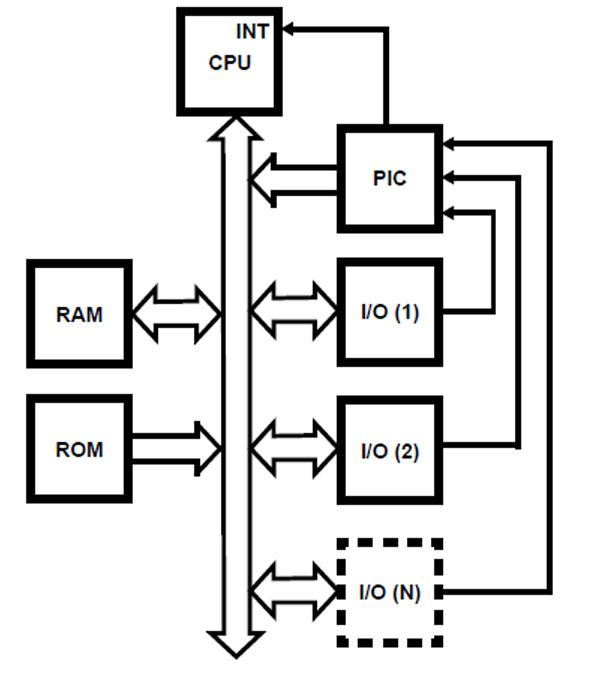
\includegraphics[width=0.5\textwidth]{img/PIC3.png}
    \caption{PIC}\label{img:PIC}
\end{figure}

Nella trattazione del PIC faremo riferimento ad un particolare chip, lo \textbf{82C59A} \ref{img:82C59A}, per la sua particolare compatibilità. Un singolo PIC può gestire fino a 8 livelli di priorità, ma è possibile creare un sistema di PIC in cascata per arrivare a gestire fino a 64 livelli di priorità. 

% Più dispositivi possono essere connessi in cascata, fino a 8 per un massimo di 64 linee di interruzione.
% Il PIC accetta richieste di interruzione dai dispositivi di IO connessi alle sue linee e determina, a seconda dell’algoritmo di gestione prioritaria selezionato, quale delle interruzioni simultaneamente attiva ha la priorità più alta. Dopodiché trasmette un segnale sulla linea INT al processore, attende un segnale su INTA (handshaking) e poi trasmette sul bus dati il vettore di 8 bit a cui corrisponde la corretta interruzione sulla tabella delle interruzioni.
% Il Control Register interno al PIC permette di configurare la gestione prioritaria mediante un’opportuna modifica:
Il PIC prevede due modalità di gestione delle priorità:
\begin{itemize}
    \item \textbf{Fully nested mode}: le richieste di interruzione sono ordinate secondo uno schema a priorità fissa che va da IR0 a IR7, con IR0 la linea più prioritaria;
    \item \textbf{Rotate mode}: Schema prioritario a rotazione (Round robin), ovvero la linea di interruzione più prioritaria appena servita diventa la meno prioritaria dopo il servizio. Da programma è possibile configurare il livello di priorità più basso.
    % \item \textbf{Maschera interruzioni} consente l’inibizione o l’abilitazione delle linee di interruzione. 
\end{itemize}

Osservando i componenti interni in figura \ref{img:82C59A}, notiamo i seguenti componenti:
\begin{itemize}
    \item \textbf{IRR}: Interrupt request register, ovvero un registro di 8 bit per ciascuna linea di interruzione in ingresso, finalizzato a memorizzare le richieste di interruzione;
    \item \textbf{ISR}: In service register, registro che memorizza i livelli di interruzione correntemente serviti;
    \item \textbf{Priority Resolver}: componente che determina le priorità delle richieste memorizzate dall'IRR e decide \textit{quale} istruzione deve essere servita, ovvero quale bit dell' ISR settare.
    \item \textbf{IMR}: Interrupt Mask Register, registro che contiene una maschera che serve a disabilitare selettivamente una o più linee di interruzione;
    \item \textbf{Bloccho R/W control}: Il blocco riceve i comandi dalla CPU per la configurazione del dispositivo e permette di “leggerne” lo stato interno;
    \item \textbf{Cascade buffer comparator}: viene utilizzato quando il PIC è collegato ad altri PIC in cascata, e le linee connesse a questo blocco servono a regolare la logica PIC master/slave.
\end{itemize}

\begin{figure}[ht]
    \centering
    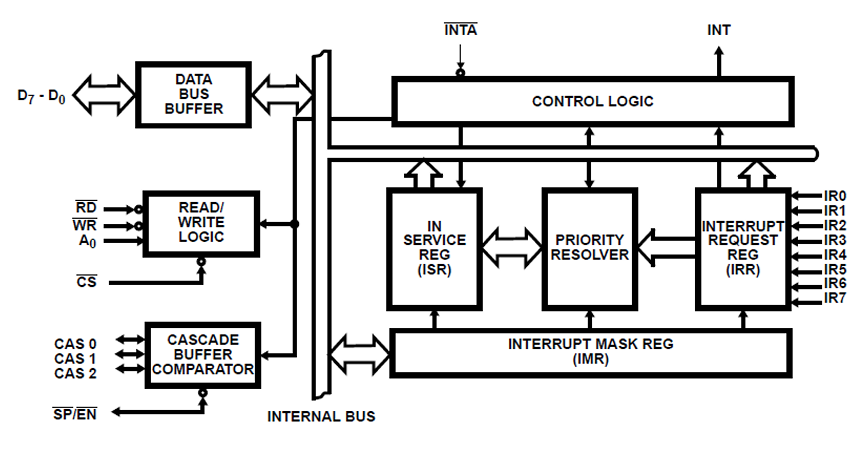
\includegraphics[width=1\textwidth]{img/PIC_82C59A.png}
    \caption{82C59A}
    \label{img:82C59A}
\end{figure}

Procediamo illustrando la modalità di funzionamento:
Inizialmente, uno o più dispositivi connessi al PIC inviano un'interruzione sulla linea alla quale sono connessi. La richiesta che arriva sulla linea i-esima, pone a 1 l'i-esimo bit del registro \textbf{IRR}. A questo punto, il \textbf{priority resolver} decide quale dispositivo deve essere servito sulla base delle priorità associate ad ogni dispositivo e in base al contenuto dell'\textbf{IMR}, e inoltra una richiesta di interruzione alla CPU (o ad un altro PIC cui è connesso in cascata) tramite la linea INT. La CPU a questo punto invia un ACK sulla linea INTA per segnalare eventualmente la disponibilità a servire l'interruzione. 
Una volta ricevuto l'ACK, il PIC setta il bit del registro \textbf{ISR} corrispondente alla linea interrompente a maggiore priorità, e resetta il corrispondente bit del registro \textbf{IRR}. Il PIC a questo punto trasmette sul \textit{bus dati} il vettore relativo al dispositivo interrompente e il bit del registro ISR corrispondente al dispositivo viene resettato. Questo ultimo reset può avvenire in due modalità:
\begin{itemize}
    \linespread{0.4}
    \item \textit{automaticamente}, se è stata selezionata la modalità \textit{automatic end of interrupt};
    \item \textit{manualmente}, settando un bit opportuno EOI tramite una parola di controllo appena prima di uscire dalla ISR. \uppercase{è} importante osservare che nel componente simulato in ASIM funziona solo questa modalità.
\end{itemize}

Attraverso i blocchi \textbf{Data Bus Buffer} (linee D0-D7) e \textbf{R/W logic} (linea $ \overline{RD}, \overline{WR}, A0, \overline{CS} $) è possibile accettare due tipi di command word proveniente dalla CPU:
\begin{itemize}
    \item \textbf{ICW}s: Initialization Command Words, che servono ad \textit{inizializzare} il dispositivo con una sequenza di minimo due e massimo quattro comandi di inizializzazione.
    \begin{itemize}
        \item \textbf{ICW1}: identificato da (A0=0,D4=1), inizia la sequenza di inizializzazione resettando il dispositivo e impostando alcuni parametri di configurazione, attraverso gli altri bit Dx.
        \item \textbf{ICW2}: segue la ICW1, identificato da A0=1, specifica i bit di indirizzo per localizzare la tabella dei vettori delle interruzioni in base al tipo di processore selezionato con la ICW1 ( 8080/85 o 80C86/88/286);
        \item \textbf{ICW3}: Identificata da A0=1, questa parola viene letta solo quando c'è più di un 82C59A in cascata, informazione acquisita attraverso la ICW1.
        \item \textbf{ICW4}: Identificata da A0=1, viene usato se in ICW1 è stato specificato IC4=1. Consente di specificare se il dispositivo deve funzionare in special fully nested mode o in buffered mode, il tipo 
        di processore con cui deve interfacciarsi, e se bisogna abilitare l'automatic end of interrupt (\textbf{AEOI}).
    \end{itemize}
    \item \textbf{OCW}s: Operation Command Words, servono a configurare la modalità di funzionamento.Dopo aver inizializzato il dispositivo con le ICW, esso è pronto ad accettare richieste di interruzione e può essere configurato con ulteriori parametri operativi:
    \begin{itemize}
        \item \textbf{OCW1}: Setta e resetta i bit della maschera nell'IMR.
        \item \textbf{OCW2}: consente di configurare il funzionamento del dispositivo per quanto riguarda la modalità \textit{end of interrupt} (permette di resettare in maniera programmatica il bit nel registro ISR) e \textit{rotate} (permette di specificare il meccanismo di rotazione delle priorità man mano che le interrupt su una linea vengono servite).
        \item \textbf{OCW3}:  consente di attivare/disattivare la special mask mode, in cui è possibile mascherare  “temporaneamente” uno specifico livello di richiesta senza avere effetto sui livelli più bassi o più alti. Il livello da mascherare è quello specificato in precedenza nella OCW1.
    \end{itemize}
\end{itemize}


Dal punto di vista esercitativo, al corso è stato presentato un componente da utilizzare nel framework ASIM che rappresenta una versione estremamente semplificata del PIC, il cui schema logico è raffigurato in figura \ref{img:piceasy}.
Il device simulato presenta 8 linee di richiesta, a ciascuna delle quali è associata una priorità fissa (modalità \textit{fully nested}), a cui possono essere connessi fino a 8 dispositivi con 8 livelli di priorità, stabiliti mediante lo schema \textit{daisy chain}. 
Il modello di programmazione del dispositivo occupa due locazioni consecutive di memoria e prevede 5 registri accessibili al programmatore. \\

\vspace{1cm}
\begin{tabular}{|p{3cm}|p{10cm}|}
    \hline
    \centering \textbf{IMR} &  (Interrupt Mask Register) permette di mascherare singolarmente le interruzioni \\
    \hline
    \centering \textbf{IRR} &  (Interrupt Request Register): memorizza i segnali di interruzione \\
    \hline
    \centering \textbf{ISR} &  (In Service Register): presenta al gestore delle interruzioni i segnali interrompenti in modo ordinato rispetto alla maschera e alla priorità corrente \\
    \hline
    \centering \textbf{CTRL} &  (Control Register): permettere di controllare il comportamento del dispositivo\\
    \hline
    \centering \textbf{TR} &  (Type Register): memorizza la parte base dell’indirizzo del vettore \\
    \hline
\end{tabular}

\vspace{1cm}
% Il modo di operazione scelto deve essere configurato in fase di inizializzazione del PIC, ma può anche essere dinamicamente cambianto da un apposito programma di gestione. Per i registri interni al PIC facciamo riferimento alla figura \ref{img:PIC2}.
% L’Interrupt Request Register (IRR) riceve in ingresso le 8 linee di interruzione provenienti dalle periferiche collegate e ne memorizza lo stato. L’input a questo registro è gestito da un circuito integrato che si occupa della gestione prioritaria delle interruzioni, mentre l’output è il registro In Service Register (ISR) in cui vengono memorizzati solo i segnali di interruzione da servire in accordo alla maschera (IMR). Il Type Register (TR) è un registro di 8 bit che memorizza nei 5 bit più significativi il valore base del vettore da scrivere in output sul bus dati, mentre nei 3 meno significativi uno spiazzamento in accordo alla linea interrompente. Dopo il servizio, l’i-esimo bit di IRR è automaticamente cancellato per riuovere la causa di interruzione.


% \begin{figure}
%     \centering
%     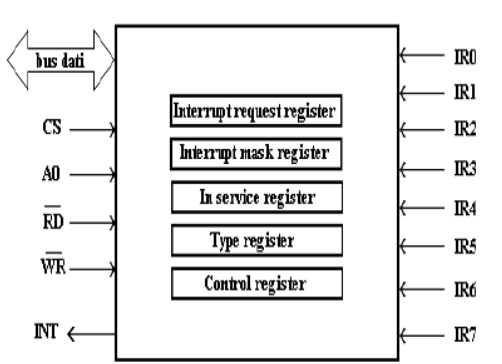
\includegraphics[width=0.5\textwidth]{img/PIC2.png}
%     \caption{PIC: modello di programmazione}\label{img:PIC2}
% \end{figure}


\begin{figure}[ht]
    \centering
    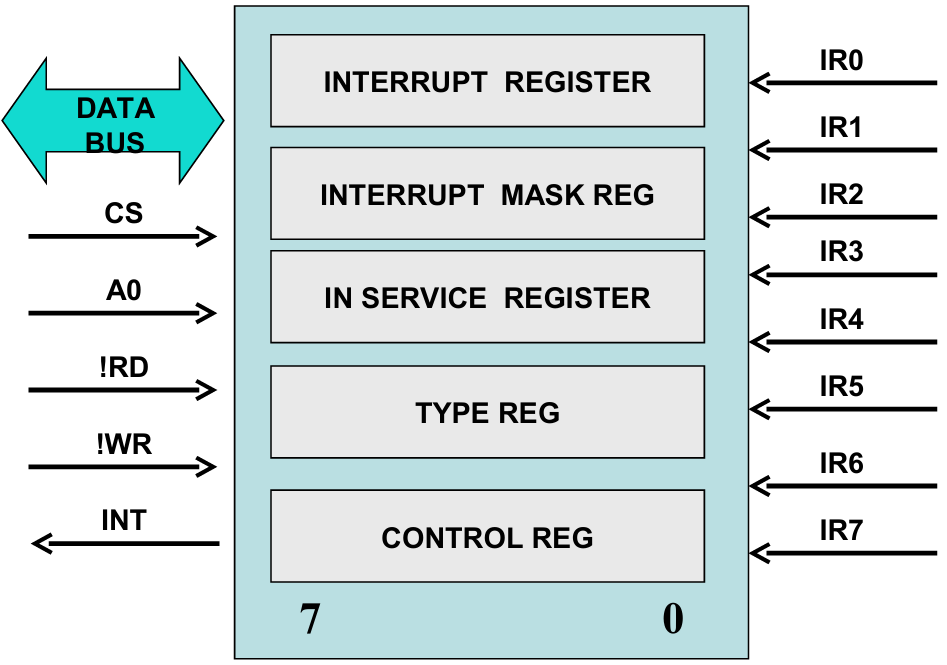
\includegraphics[width=0.7\textwidth]{img/easy_pic.png}
    \caption{PIC semplificato}
    \label{img:piceasy}
\end{figure}

Vediamo nel dettaglio il funzionamente di questi registri:
\begin{itemize}
    \item \textbf{TYPE REGISTER}: contiene informazioni sui vettori di interruzione associati al PIC. I vettori si ricavano a partire da un \textit{vector number} di base sommando uno spiazzamento su 3 bit, ovvero i 3 bit meno significativi del registro. Lo spiazzamento viene settato automaticamente in base alla linea interrompente. Praticamente al programmatore è permesso di inserire il numero di base, al quale viene automaticamente sommato uno spiazzamento in base alle linea interrompente.  L’accesso a TR viene fatto selezionando in scrittura  l’indirizzo dispari subito dopo un \textit{RESET};
    \item \textbf{INTERRUPT MASK REGISTER}: memorizza le linee di interruzione che devono essere mascherate. Per mascherare una linea basta inserire un 1 nel bit corrispondente. IMR è accessibile sia in lettura che in scrittura ad indirizzo dispari, ma in scrittura il dispositivo non deve essere nello stato \textit{reset}, ovvero deve essere già stato scritto almeno TR;
    \item \textbf{CONTROL REGISTER}: registro da 8 bit accessibile sempre in scrittura ad indirizzo pari:
    \begin{itemize}
        \item bit 0,1,2: determinano il bit da cancellare in \textit{ISR}.
        \item bit 3: bit End of Interrupt, se posto a 1 fa cancellare il bit puntato dai bit 0-2. 
        \item bit 4: bit Automatic End of Interrupt, se posto a 1 fa cancellare automaticamente il bit in ISR dopo la trasmissione dell'interruzione;
        \item bit 5: \textit{non utilizzato};
        \item bit 6: bit Register Interrupt Selector, se il bit 7 è alto seleziona l'accesso a ISR in lettura, se il bit 7 è basso seleziona l'accesso a IRR in lettura;
        \item bit 7: permette se posto a 1 la lettura dei registri ISR e IRR (vedi punto precedente).
    \end{itemize}
    \item \textbf{INTERRUPT REQUEST REGISTER}: memorizza le richieste di interruzione relative alle singole linee di interruzione. Questo registro è accessibile solo in lettura ad indirizzo pari in accordo a quanto scritto nel registro CTRL. 
    Quando la richiesta d'interruzione, arrivata sulla linea n, viene spedita al gestore delle interruzioni (PIC o CPU) collegato al PIC, il bit n-esimo di IRR è cancellato;
    \item \textbf{IN SERVICE REGISTER}: sono memorizzate le interruzioni trasmesse.  Questo registro è accessibile solo in lettura all'indirizzo pari in accordo con quanto settato nel registro di controllo. 
\end{itemize}

\subsection{Estensione del modello IO generale}
Un modello di architettura dotato solo di PIA (\ref{par:PIA}) è limitato: può gestire solo caratteri, ha a disposizione solo 7 interruzioni e può generare attese infinite con il protocollo di handshaking.
Per risolvere questi problemi, vengono introdotti nuovi elementi nell'architettura: \textbf{DMA} per gestire il trasferimento di messaggi invece di caratteri, \textbf{PIC} (\ref{par:PIC}) per superare la limitazione sul numero di ISR indirizzabili e \textbf{TIMER} per gestire la temporizzazione e il risolvere il problema delle attese infinite (\ref{img:IO_ESTESO}).

\begin{figure}[ht]
    \centering
    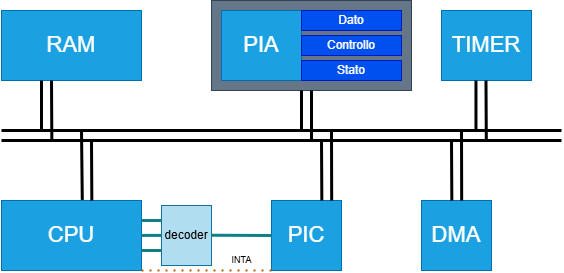
\includegraphics[width=0.75\textwidth]{img/Schema_IO_1.png}
    \caption{Modello IO esteso - schema logico}
    \label{img:IO_ESTESO}
\end{figure}

Il timer espone il modello di programmazione Registro di stato, Registro di valore e Registro di Modo. Nel registro di valore di solito è scritto un istante in cui il timer si "sveglia" e genera un'interruzione: infatti il timer possiede una linea con la quale può comunicare un'interruzione.
